\documentclass{article}
\usepackage[utf8]{inputenc}

\title{Laboratorio03_INTELIGENCIA_NEGOCIOS}
\author{edwartbalcon}
\date{Septiembre 2021}

\usepackage[utf8]{inputenc}
\usepackage[spanish]{babel}
\usepackage{natbib}
\usepackage{graphicx}

\begin{document}

\title{Caratula}

\begin{titlepage}
\begin{center}
\begin{Large}
\textbf{UNIVERSIDAD PRIVADA DE TACNA} \\
\end{Large}
\vspace*{-0.025in}
\begin{figure}[htb]
\begin{center}

\includegraphics[width=6cm]{./images/logo_UPT}
\end{center}
\end{figure}
\vspace*{-0.025in}
\begin{Large}
\textbf{FACULTAD DE INGENIERIA} \\
\end{Large}
\vspace*{0.05in}
\begin{Large}
\textbf{Escuela Profesional de Ingeniería de Sistema} \\
\end{Large}


\vspace*{0.4in}

\vspace*{0.1in}
\begin{Large}
\textbf{Informe de laboratorio 08: Lambda, Kinesis Data Streams,
DynamoDB, SNS, EC2, IAM} \\
\end{Large}

\vspace*{0.3in}
\begin{Large}
\textbf{Curso: Inteligencia de negocios} \\
\end{Large}

\vspace*{0.3in}
\begin{Large}
\textbf{DOCENTE: Ing. Patrick Cuadros Quiroga} \\
\end{Large}

\vspace*{0.2in}
\vspace*{0.1in}
\begin{large}

\begin{Large}
\textbf{Alumno: Balcon Coahila, Edwart Juan\hfill	(2013046516) } \\
\end{Large}

\vspace*{0.15in}
\begin{Large}
\textbf{Tacna – Perú} \\
\end{Large}

\vspace*{0.05in}
\begin{Large}
\textbf{2021 } \\
\end{Large}

\end{large}
\end{center}

\end{titlepage}


\newpage

\section{ Realizar los siguientes pasos para el laboratorio }

\textbf{1.1.  Accedemos a Cloud9}

	
\textbf{1.2. Creamos el recurso en Kinesis Data Streams y la tabla en DynamoDB mediante CloudFormation}


    \begin{center}
		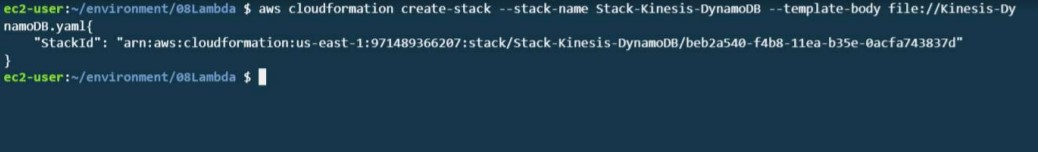
\includegraphics[width=15cm]{./images/1} 
	\end{center}

\textbf{1.3.   Clic en Crear una función
}

    \begin{center}
		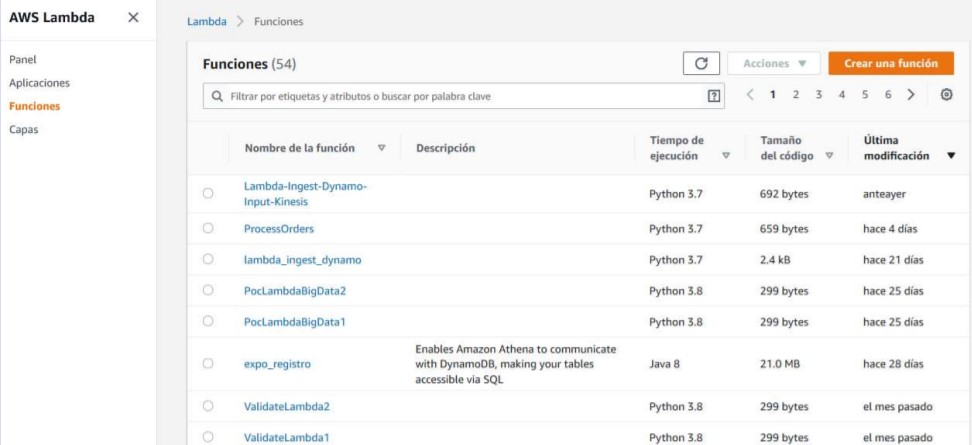
\includegraphics[width=15cm]{./images/2} 
	\end{center}

\newpage
\textbf{1.4.  El nombre de la función será (opcional): WriteDynamoDBSendSNS
El lenguaje de programación será Python 3.8
Clic en Crear una función
}

    \begin{center}
		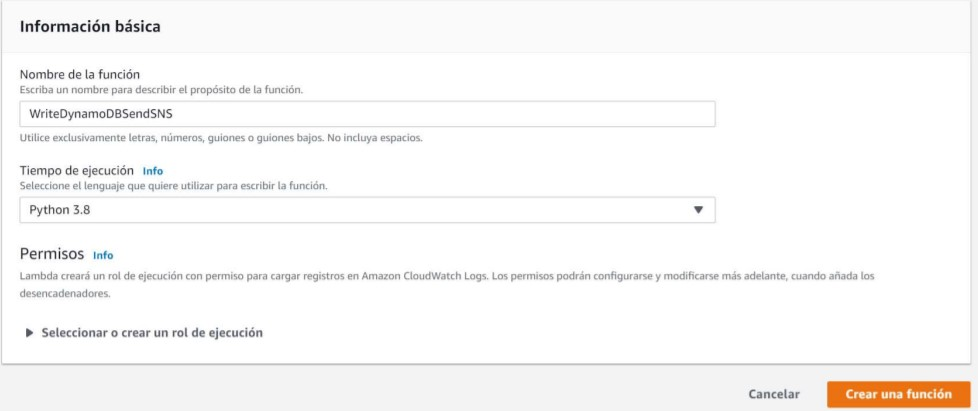
\includegraphics[width=15cm]{./images/3} 
	\end{center}
	
	\newpage
\textbf{1.5.   Ir al servicio de SNS, agregar el nombre : topicProduct y paso siguiente
}

    \begin{center}
		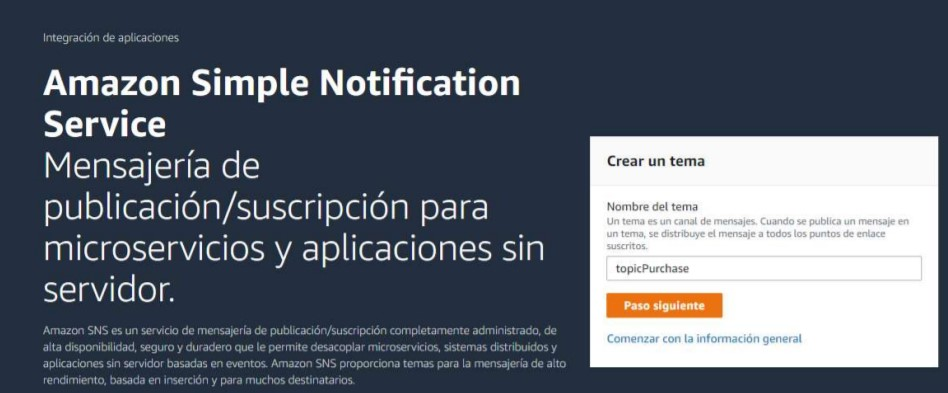
\includegraphics[width=15cm]{./images/4} 
	\end{center}
	
	\newpage
\textbf{1.6.   Crear una suscripción
Clic en Crear una suscripción
}

    \begin{center}
		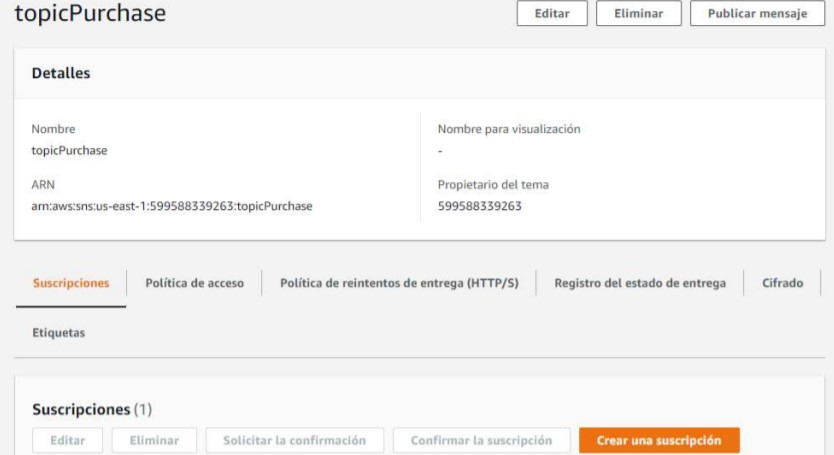
\includegraphics[width=15cm]{./images/5} 
	\end{center}
	 \begin{center}
		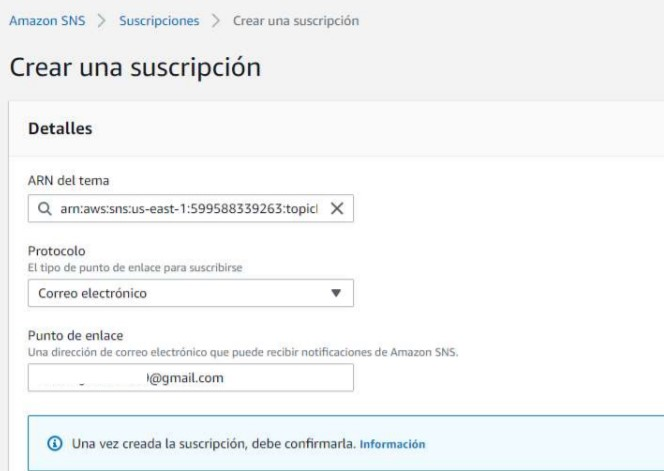
\includegraphics[width=15cm]{./images/6} 
	\end{center}
	
	\newpage
\textbf{1.7. Nos llegará un correo para confirmar la suscripción al tópico, y poder recibir correo por el servicio
de SNS:
}

    \begin{center}
		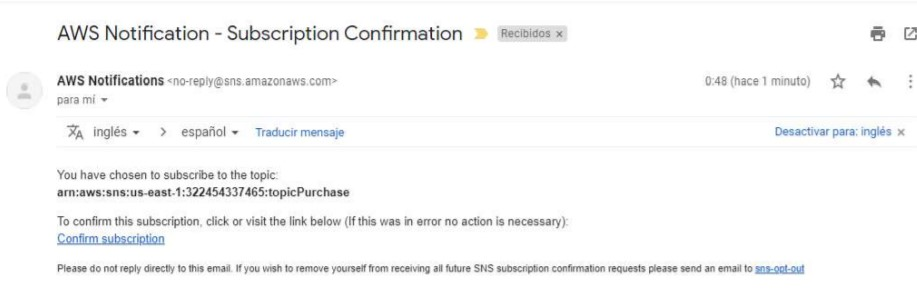
\includegraphics[width=15cm]{./images/7} 
	\end{center}
	
	\newpage
\textbf{1.8.  Y procedemos a confirmar:
}

    \begin{center}
		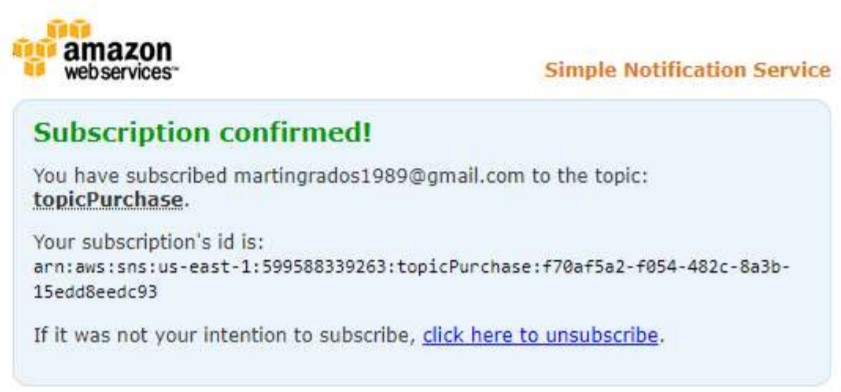
\includegraphics[width=15cm]{./images/8} 
	\end{center}
	
    \begin{center}
		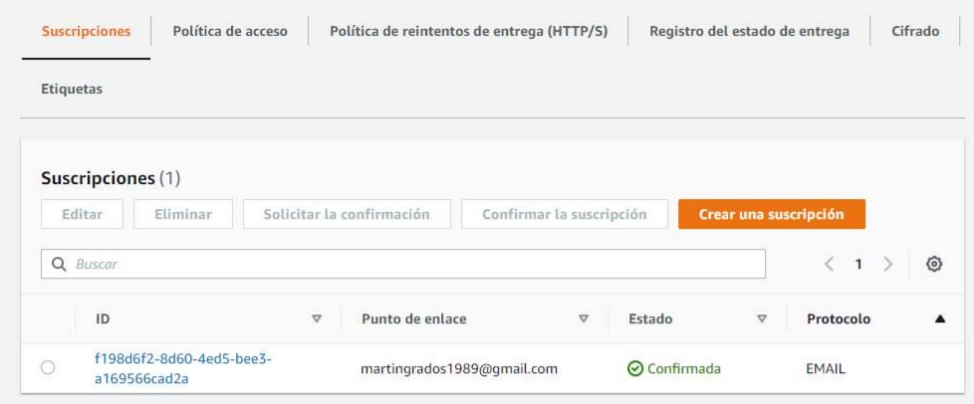
\includegraphics[width=15cm]{./images/9} 
	\end{center}
	
	\newpage
\textbf{1.9.   Actualizar el rol, entrar a la función Lambda WriteDynamoDBSendSNS
Clic donde se indica la flecha.
}

    \begin{center}
		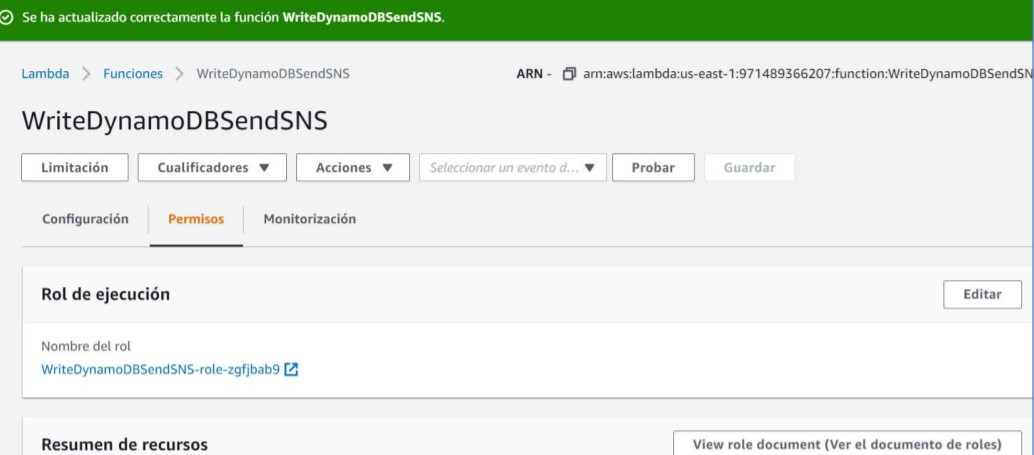
\includegraphics[width=15cm]{./images/10} 
	\end{center}
	
		
	\newpage
\textbf{1.10.  Clic en la opción de expandir.
}

    \begin{center}
		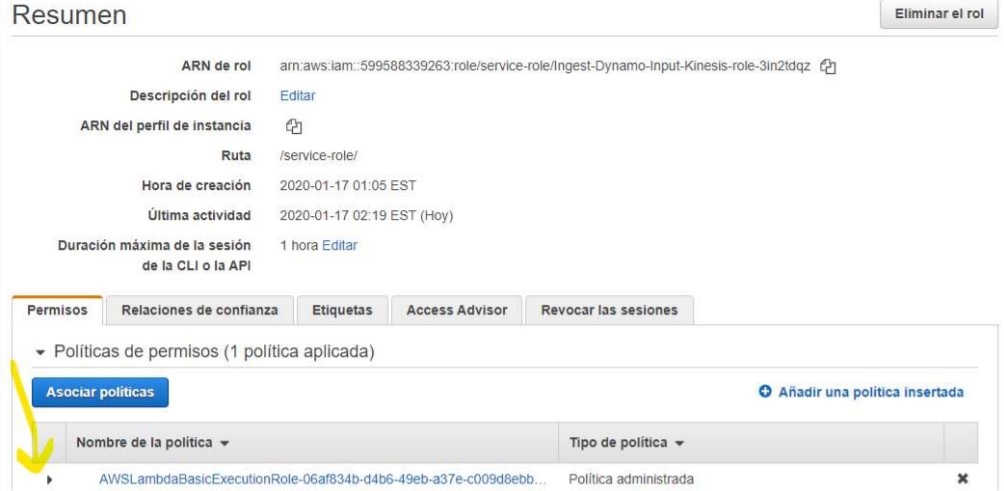
\includegraphics[width=15cm]{./images/11} 
	\end{center}
	
	
		
	\newpage
\textbf{1.11.  Editar la Politica:
}

    \begin{center}
		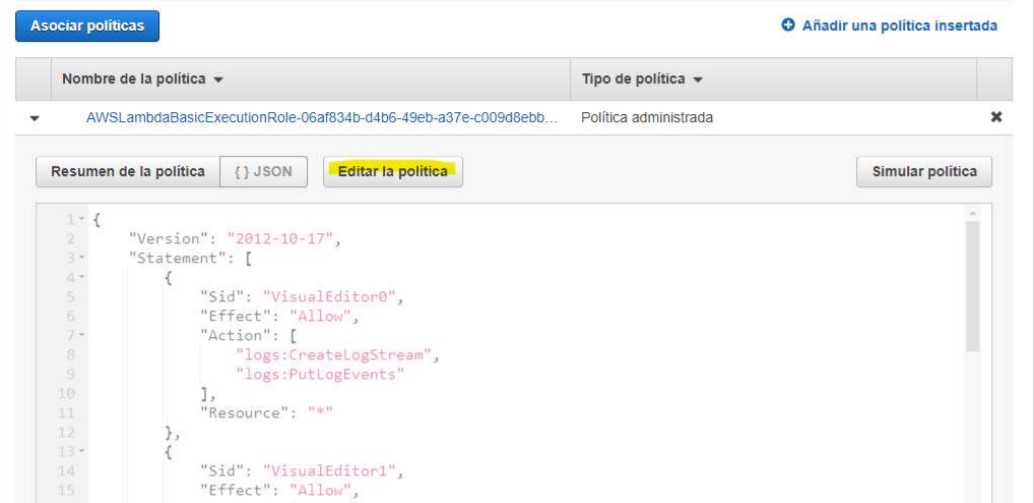
\includegraphics[width=15cm]{./images/12} 
	\end{center}
	
	
	\textbf{1.12.  Click en la opción de JSON:
}

    \begin{center}
		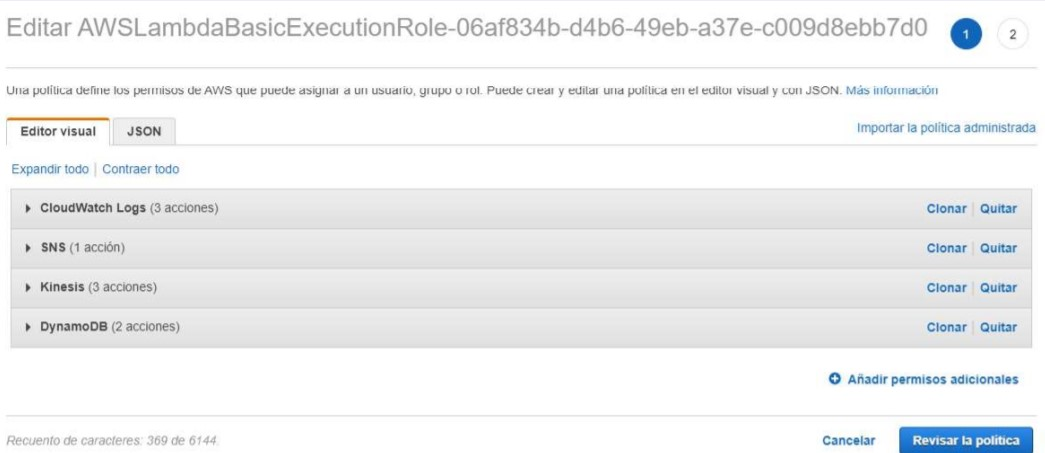
\includegraphics[width=15cm]{./images/13} 
	\end{center}
	
	\textbf{1.13.  Agregar el desencadenador de Kinesis.
}

    \begin{center}
		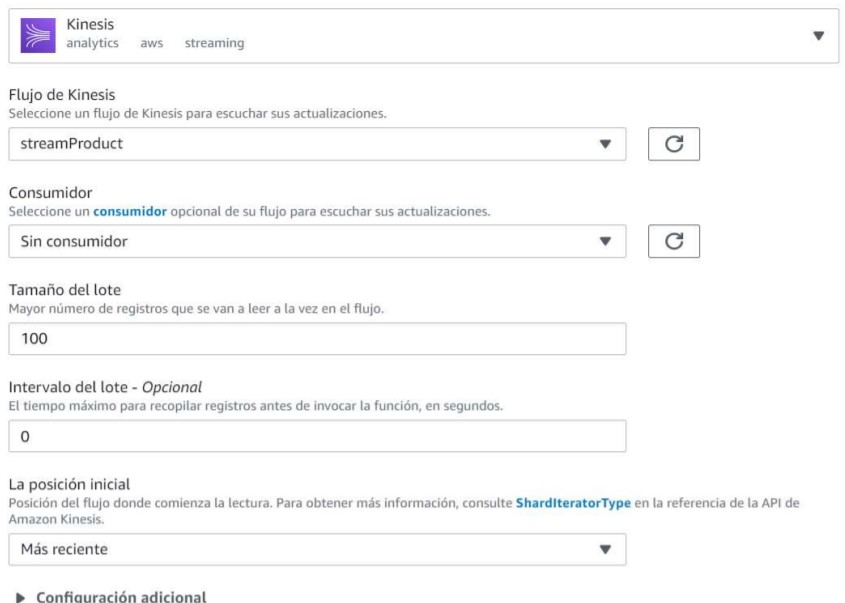
\includegraphics[width=15cm]{./images/14} 
	\end{center}
	
	\textbf{1.14.  Ejecutar el archivo Python
python3 WriteKinesisProduct.py 
}

    \begin{center}
		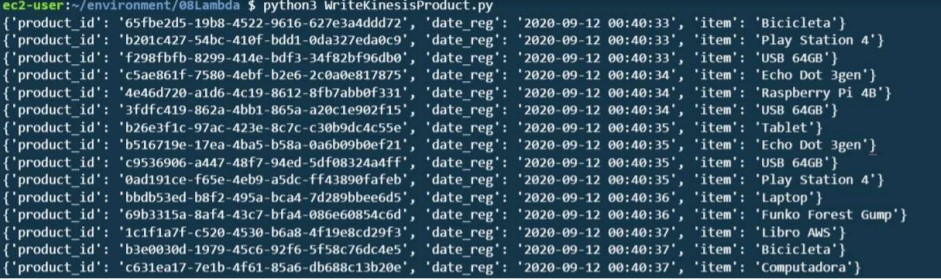
\includegraphics[width=15cm]{./images/15} 
	\end{center}
	
	\textbf{1.15.  Verificar que se hayan ingestado los datos a DynamoDB y si se tiene dentro de la compra una
Raspberry Pi 4B debe llegar un mensaje de correo.
}

    \begin{center}
		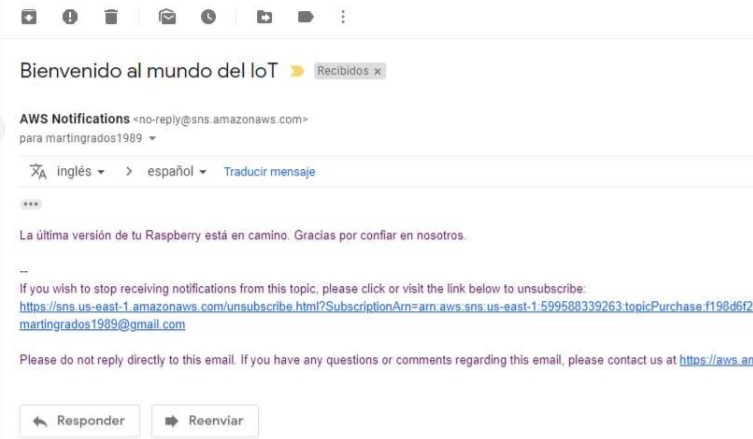
\includegraphics[width=15cm]{./images/16} 
	\end{center}
	
	\textbf{1.16.  Verificamos los datos en la tabla de DynamoDB
}

    \begin{center}
		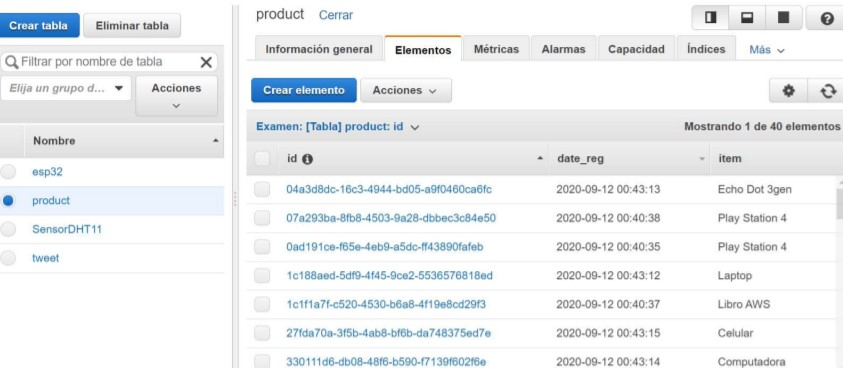
\includegraphics[width=15cm]{./images/17} 
	\end{center}
	
\end{document}